\section{Experimental Evaluation}\label{sec:exp}


We evaluate our techniques on two real-world trajectory datasets: \pt{} and \sz{}.
\pt{}~\cite{pt} contains a total of 2.39 million taxi trajectories and 75.67 million of GPS points, and the longest trajectory has 3,490 GPS points.
\sz{}~\cite{sz} consists of 3.07 million taxi trajectories with 53.53 million GPS points, and the longest trajectory has 2,268 GPS points. All experiments are conducted on a machine with an Intel i7-8700 CPU, 24 GB memory and an NVIDIA GeForce GTX1080 GPU with 8 GB on-chip memory, running on Windows 10. All methods are implemented in Java 1.8, and the Processing 3 library~\cite{p3} is used for rendering. All datasets and source codes required to reproduce our results are available at~\cite{code}.

\REPORT{
This section is organized as follows. 
In Section~\ref{sec:case}, we present several case studies of the visualization results on the \pt{} and \sz{} datasets to demonstrate the merits of our methods.
% In Section~\ref{sec:case}, we evaluate the effectiveness of our proposal by the case studies on \pt{} and \sz{} trajectory dataset, respectively.
}
In Section~\ref{sec:user}, we conduct a comprehensive user study to test the effectiveness of our visualization results on practical  tasks including \textit{region center identification}, \textit{reachable route inspection} and \textit{traffic flow comparison}. In Section~\ref{sec:quality}, we quantitatively evaluate the fidelity loss and efficiency of our methods.

% and has been cleaned for further analysis.

\subsection{Case Study of Visualization Results}\label{sec:case}

\subsubsection{Case Study on Porto}\label{sec:pt}
% We demonstrate the effectiveness of our proposal by the case studies in \pt{} in Section~\ref{sec:pt} and \sz{} {in Section~\ref{sec:sz}}.

% \subsubsection{Case Studies on \pt{}}\label{sec:pt}
%For the sake of page limitation, we omit the detail elaboration of the cases in Figure~\ref{fig:teaser} and refer the interested reader to our technical report~\cite{techreport}.
%In this section, we present the effectiveness of our proposals with different detail views by investigating three regions of interest in \pt{}, as R1, R2, and R3 shown in Figure~\ref{fig:porto}(A).

We use the visualization results in Figure~\ref{fig:teaser} to demonstrate the effectiveness our proposals from the following three aspects.


\stitle{Consistently good visual fidelity at different zoom-levels}
At zoom level 11, Figure~\ref{fig:teaser}(A) is the visualization result of the full \pt{} dataset.
With a sampling rate $\alpha \!=\! 1\%$, Figures~\ref{fig:teaser}(C) and (E) are the visualizations produced by uniform random sampling ($\rand$)
and our advanced visual fidelity-guaranteed sampling method ($\avats$, Algorithm~\ref{alg:plus}), respectively. Comparing with Figure~\ref{fig:teaser}(C), it is obvious that Figure~\ref{fig:teaser}(E) is more similar to Figure~\ref{fig:teaser}(A). In particular, Figure~\ref{fig:teaser}(E) not only preserves the overall visual structure of the entire region but also keeps the details of cities that are far from the center (marked by the dashed cycles in the figure). However, the details of these cities are lost in Figure~\ref{fig:teaser}(C) as $\rand{}$ mostly samples trajectories in the dense region.

Figures~\ref{fig:teaser}(H) and (I) are the visualizations generated by $\rand$ and $\avats$  (with color encoding), respectively, at zoom level 15 with a sampling rate $\alpha=1\%$.
Compared with the visualization using the full dataset at this level (i.e., Figure~\ref{fig:teaser}(G)), Figure~\ref{fig:teaser}(H) only shows a few trajectories and most of the information in the raw data is lost. In contrast, Figure~\ref{fig:teaser}(I) captures the overall structure of Figure~\ref{fig:teaser}(G), and the details are even clearer than Figure~\ref{fig:teaser}(G) thanks to color encoding.

%We will show in Section 6.3 that our visual fidelity loss reduces when sampling rate increases, which indicates the visual fidelity loss is an effective measure.

\stitle{Consistently good visual fidelity under different sampling rates}
Figures~\ref{fig:teaser}(B) and (C) are the visualizations produced by $\rand{}$ with a sampling rate of $0.1\%$ and $1\%$, respectively, while Figures~\ref{fig:teaser}(D) and (E) are the visualizations generated by our $\avats{}$ algorithm at the same sampling rates. We can make two observations: (i) the larger the sampling rate, the better the visual fidelity, i.e., Figures~\ref{fig:teaser}(C) and (E) are more similar to Figure~\ref{fig:teaser}(A) compared with Figures~\ref{fig:teaser}(B) and (D); (ii) the visualization of $\avats$ with a sampling rate of $0.1\%$ (i.e., Figure~\ref{fig:teaser}(D)) looks even more appealing than the visualization of $\rand{}$ with a sampling rate of $1\%$ (i.e., Figure~\ref{fig:teaser}(C)) as Figure~\ref{fig:teaser}(D) better captures the overall visual structure of Figure~\ref{fig:teaser}(A).

\stitle{Color encoding effectively mitigates visual clutter}
% Then, we present the superiority of the color encoding scheme in $\avats$, which denotes as $\cavats$ in subsequent sections.
At a zoom level of 11 and with a sampling rate of $1\%$, Figures~\ref{fig:teaser}(E) and (F) are the visualizations produced our $\avats$ and $\cavats$ (i.e., $\avats$ with color encoding), respectively.
Visual clutter is severe for the full dataset (i.e., Figure~\ref{fig:teaser}(A)) and Figures~\ref{fig:teaser}(E), and it is difficult to identify a specific trajectory in the dense region. The visualization of $\cavats$ in Figure~\ref{fig:teaser}(F) reduces the visual clutter by encoding the trajectories with color, and thus it is easy to identify some prominent trajectories. The comparison between Figure~\ref{fig:teaser}(G) (full dataset) and Figure~\ref{fig:teaser}(I)  ($\cavats$) at a sampling rate of $0.1\%$ also validates the effectiveness of color encoding.

\begin{figure*}[t]
	\centering
	\includegraphics[width=0.95\textwidth]{pictures/experiment_study/case_porto.pdf}
	\vspace{-3mm}
	\caption{Effectiveness studies of $\avats$ at dense and sparse regions with detail visualizations in \pt{}.}
	\label{fig:porto}
	\vspace{-2mm}
\end{figure*}

\REPORT{
We next present the effectiveness of our proposals with different detail views by investigating three regions of interest in \pt{}, as R1, R2, and R3 shown in Fig.~\ref{fig:porto}(A).

\stitle{Sparse region R1}
R1 is a sparse region and has few trajectories, as the visualization result of full \pt{} dataset shown in Fig.~\ref{fig:porto}(B1).
The reason is the two cities Paredes and Penafiel in R1 are far away from the center of Porto.
Given sampling rate $\alpha=0.5\%$, Fig.~\ref{fig:porto}(B2), (B3) and (B4) are the visualization results of the returning trajectory set from $\rand{}$, $\vats$ and $\avats$ with $\delta=64$, respectively.
As our above statement, the result of $\rand$ almost misses all information in sparse region.
While $\vats$ performs much better than $\rand$ as it provides theoretical visual fidelity guarantee, but it still lost detail information.
Taking Fig.~\ref{fig:porto}(B1) as reference, the trajectory bundle and trajectory structure are lost in Fig.~\ref{fig:porto}(B3$a$) and (B3$b$).
As expected, our advanced approach $\avats$ in Fig.~\ref{fig:porto}(B4) with perception tolerance value $\delta=64$ did an excellent job to capture the details in the full dataset when comparing with $\vats$ in Fig.~\ref{fig:porto}(B3).
As shown in Fig.~\ref{fig:porto}(B4$b$), the trajectory sketch of Penafiel is almost the same as it in Fig.~\ref{fig:porto}(B1$b$), the visualized result of full dataset.



\stitle{Median region R2} It is near to the center of Porto, which has more taxi trajectories than R1, see Fig.~\ref{fig:porto}(A).
As noted in Fig.~\ref{fig:porto}(C1), R2 includes three cities: Ermesinde, Rio Tinto and Valongo.
Fig.~\ref{fig:porto}(C2) and (C3) visualized the returning result of $\avats$ with perception tolerance value $\delta=4$ and $64$, respectively.
Visually, Fig.~\ref{fig:porto}(C3) has more trajectory branch details than Fig.~\ref{fig:porto}(C2), as the rectangles $c$ and $d$ shown in them.
%It shows that the larger perception tolerance value, the more details in this region reserved at zoom level 14.
%Comparing with Fig.~\ref{fig:porto}(C3),
Fig.~\ref{fig:porto}(C4) is the result of $\cavats$, i.e., it colors the trajectories by their representativeness.
Intuitively, Fig.~\ref{fig:porto}(C4) shows its superiority over Fig.~\ref{fig:porto}(C3) to capture the trajectory distributions.
For example, the color of the region $f$ in Fig.~\ref{fig:porto}(C4) is {darker} than the rest two regions $e$ and $g$.
Thus, we can conclude Rio Tinto (region $f$) has more taxi trajectories than other two cities, which is hard to be concluded via Fig.~\ref{fig:porto}(C3), even Fig.~\ref{fig:porto}(C1), the visualization result of full dataset.
It verified that the color encoding scheme could enrich the visual information in large trajectory visualization.

\stitle{Dense region R3} It is the center of Porto, which has the highest concentration of the trajectories and causes serious visual clutter, as visualized in Fig.~\ref{fig:porto}(D1).
For example, the structure of trajectories in Fig.~\ref{fig:porto}(D1$i$) is unclear.
$\avats$ with $\delta=4$ alleviates the visual clutter and preserves the trajectory distribution, see Fig.~\ref{fig:porto}(D2).
Fig.~\ref{fig:porto}(D3) visualized the result of $\avats$ with $\delta=64$, which enhances the visual fidelity of Fig.~\ref{fig:porto}(D2).
Specifically, it preserves more details (see rectangle $h$) and has a more clear structure in the {densest} region (see rectangle $i$).
Visually, Fig.~\ref{fig:porto}(D4) is the best among these four visualization results.
It confirms the advantages of color encoding scheme in $\cavats$.



\vspace{-2mm}

\subsubsection{Case Studies on \sz}\label{sec:sz}
We further evaluate the effectiveness of our approaches by using the taxi trajectories in Shenzhen, China.
The \sz{} trajectory dataset has many different characteristics with \pt{}, e.g., trajectory distribution, city centers, and taxi move patterns.
We set sampling rate $\alpha=1\%$ and perception tolerance value $\delta = 64$ in this section.

\begin{figure*}[t]
	\centering
	\includegraphics[width=0.95\textwidth]{pictures/experiment_study/case_shenzhen.pdf}
	\vspace{-4mm}
	\caption{Case studies on \sz{} taxi trajectory dataset, sampling rate $\alpha = 1\%$.}
	\label{fig:shenzhen}
	\vspace{-3mm}
\end{figure*}

\stitle{Overview of Shenzhen}
Fig.~\ref{fig:shenzhen}(A) is the visualization result of full \sz{} dataset at zoom level 11.
The dense regions in southern of Shenzhen, as the dashed circles shown in Fig.~\ref{fig:shenzhen}(A), are \emph{Baoan, Nanshan, Futian} and \emph{Luohu} districts,
which are the most prosperous commercial regions in this city.
The returning results of $\rand$, $\avats$ and $\cavats$ are visualized in Fig.~\ref{fig:shenzhen}(B), (C) and (D), respectively.
Not surprisingly,  the visualized result of $\rand$ in Fig.~\ref{fig:shenzhen}(B) is quite different from the full dataset in Fig.~\ref{fig:shenzhen}(A).
$\avats$ in Fig.~\ref{fig:shenzhen}(C) shows it superiority by capturing the overview of \sz{} dataset and even preserves the isolated trajectories,
as highlighted in left-upper corner of Fig.~\ref{fig:shenzhen}(C).
It owes to $\avats$ provides theoretical visual fidelity guarantees on the returning result set.
$\avats$ with color encoding $\cavats$ further improved the visual fidelity of $\avats$.
Specifically, both Fig.~\ref{fig:shenzhen}(A) and (C) are suffering from visual clutter seriously,
e.g., it is unable to recognize the main roads in the circles $a$ and $b$ as both are full with trajectories.
However, the result of $\avats$ with color encoding, as shown in Fig.~\ref{fig:shenzhen}(D), reduce the visual clutter perfectly.
For example, it is clear that the main roads of circle a and b are these roads with {darker} colors in Figure~\ref{fig:shenzhen}(D).

We then present the advantages of our $\avats$ in two representative areas, i.e., airport and North railway station, in \sz{} dataset.

\stitle{Airport in Shenzhen}
Comparing with visualization result of full dataset in Fig.~\ref{fig:shenzhen}(E),
the visualized result of $\rand$ in Fig.~\ref{fig:shenzhen}(F) only includes very few trajectories.
both $\avats$ and $\cavats$ (see Fig.~\ref{fig:shenzhen}(G) and (H)) reserve the major structure of the airport area excellent.
Moreover, $\cavats$ provides richer information by computing the representativeness of trajectories.
For example, the taxi trajectories which pass through G4 and G104 is more than that in Baoan Avenue.
The reason is that the colors of G4 and G104 is {darker} than Baoan Avenue, as highlighted in Fig.~\ref{fig:shenzhen}(H).


\stitle{North railway station in Shenzhen}
We next investigate the visualizations of the full dataset, uniform random sampling result set, and visual fidelity guaranteed sampling result set around North railway station of Shenzhen, which are shown from Fig.~\ref{fig:shenzhen}(I) to (L).
Interestingly, $\avats$ and $\cavats$ visualized the overpass near North railway state clearly, as circle $c$ shown in both Fig.~\ref{fig:shenzhen}(K) and (L).
Due to visual clutter, the overpass is not clear in Fig.~\ref{fig:shenzhen}(I), which visualized the full dataset.
It even disappeared in the visualized result of $\rand$ in Fig.~\ref{fig:shenzhen}(G).
Moreover, it is easy to compare the traffic flows in different roads via $\cavats$ visualization result.
For example, the road G94 has a higher road traffic flow than the Minzhi Avenue and Meilong Avenue, as different colors shown in Fig.~\ref{fig:shenzhen}(L).
}



\subsection{User Study for Practical Tasks}\label{sec:user}

In this part, we evaluate the effectiveness of our proposals by recruiting 186 participants to conduct practical spatial tasks. These spatial tasks (illustrated in Figure~\ref{fig:apps}) are designed by our industry partner, Tencent Map~\cite{tencentmap}, according to their user study. The results show that our algorithms provide informative visualizations, which lead to good user performance in these tasks.

\begin{figure}[t]
	\centering
	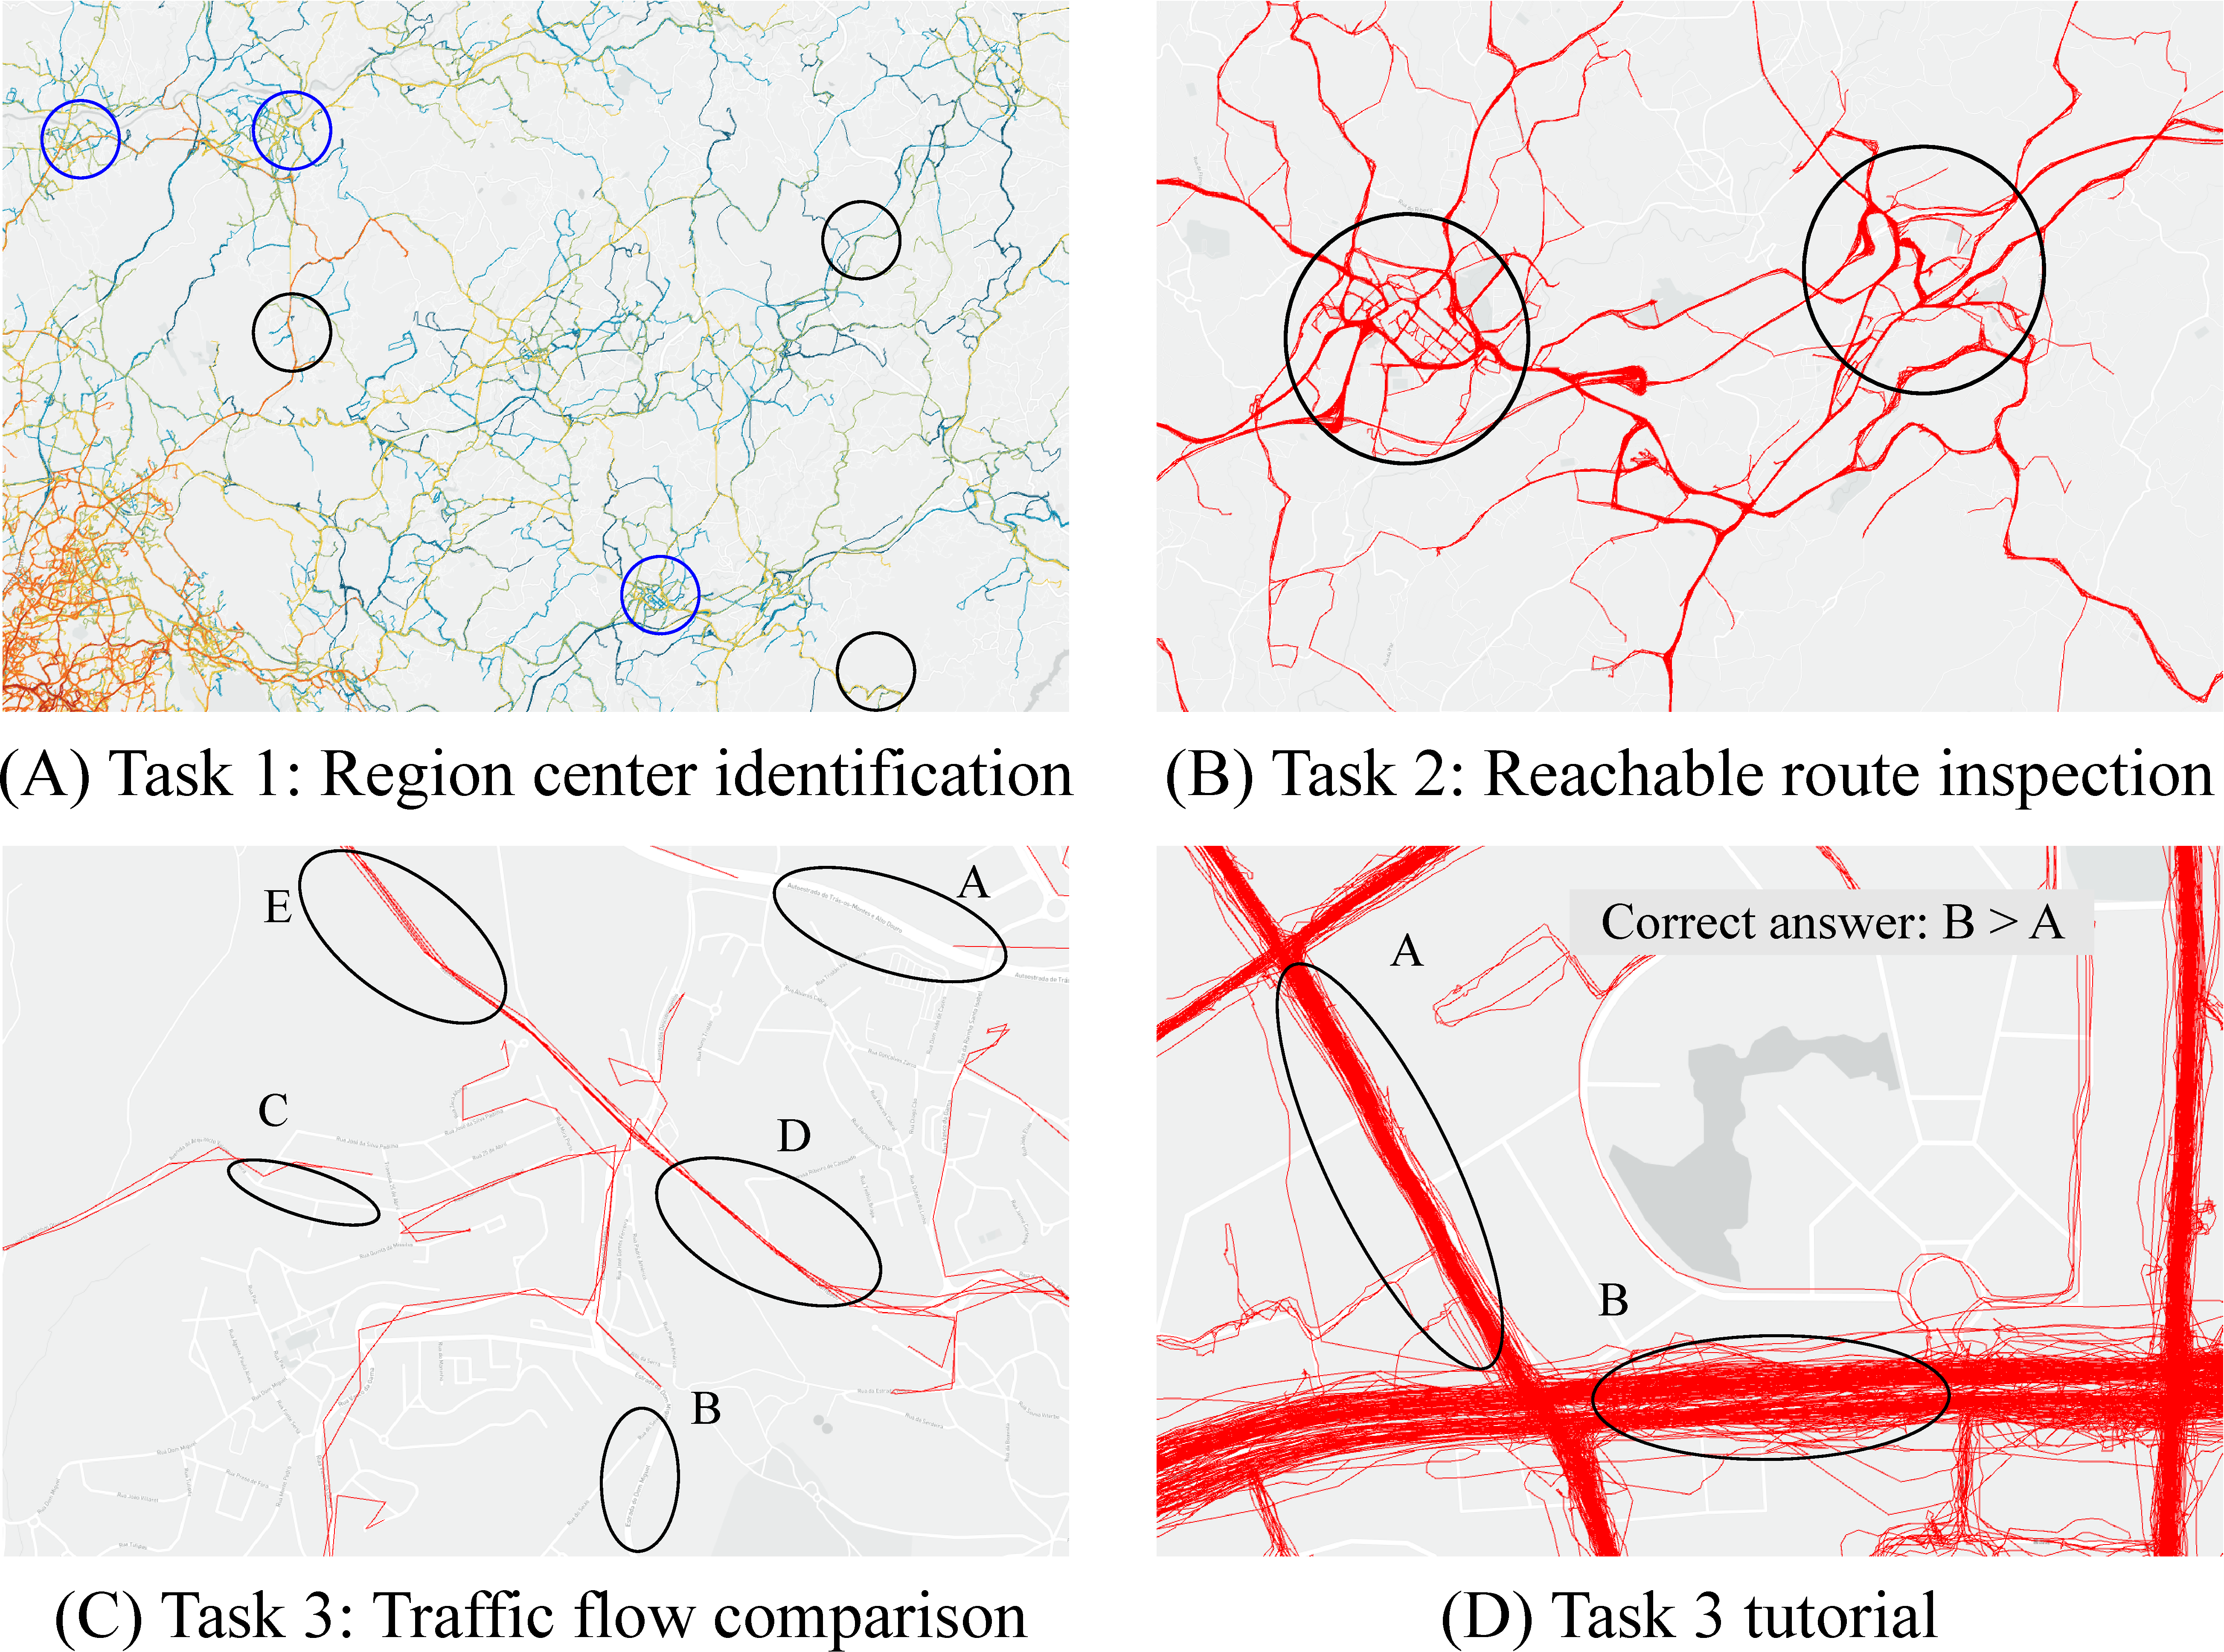
\includegraphics[width=0.45\textwidth]{pictures/user_study/interface.pdf}
	\vspace{-3mm}
	\caption{The three tasks in the user study.}
	\label{fig:apps}
	\vspace{-4mm}
\end{figure}

%\subsubsection{Settings}\label{sec:uset}

\stitle{Settings}
We recruited 186 participants with 24 females, 162 males, aged 18-29 with a mean of 21.16 for the user study\footnote{We are aware of the gender and age bias in the participants as we mainly recruited students from a university due to some practical constraints. However, we think the test results are still informative as we observed that the performance of a participant in the tasks is not significantly affected by these factors.}. The user study system is a web-based platform, in which all visualizations are displayed with a resolution of 450*300. We used the two taxi trajectory datasets, i.e., \pt{} and \sz{}, to generate the visualizations.


We test five visualization methods: (i) exact visualization using the full dataset, denoted as $\full$; (ii) uniform random sampling, denoted as $\rand$; (iii) our $\vats$ algorithm; (iv) our $\avats$ algorithm; (v) $\avats$ with color encoding, denoted as $\cavats$. The sampling rate is $\alpha = 0.5\%$ for $\rand$ and our algorithms, and $\delta = 64$ for $\avats$ and $\cavats$. The tasks are described as follows:


\textit{(T1): region center identification.} The downtown areas or commercial regions of a city are hubs for human activities and crucial for traffic management. We also observed that the taxi trajectories are denser in these regions than the other regions for both datasets. T1 contains 30 visualizations of six selected regions, which include city or commercial centers from the \pt{} dataset. For each visualization, we manually label three locations as region centers, and randomly generate three locations far away from the correct centers as fake centers. Each participant is asked to check six randomly selected visualizations and choose three region centers from each visualization, as illustrated in Figure~\ref{fig:apps}(A).

%We are interested in the average user accuracy under different visualization methods.


\textit{(T2): reachable route inspection.} Visualized trajectories should show reachable routes that connect different regions and allow users to identify them. In this task, a participant is presented with a visualization containing two circular areas (as shown in Figure~\ref{fig:apps}(B)) and asked to draw the representative reachable routes between the two areas. We assume that a route is more representative if there are a larger number of trajectories containing it. For each visualization, we manually generate at least 5 reachable routes and a user answer is considered correct if it contains 3 of these routes. T2 includes 35 visualizations of seven different regions, and for each visualization, two cities/commercial districts are marked by circles. Each participant is asked to check five randomly selected visualizations.


\textit{(T3): traffic flow comparison.} A road with a large traffic flow (i.e., having many trajectories passing it) should have dense and broad trajectory brunch in the visualization. For the $\avats$ algorithm with color encoding, such large track flow can also be identified by the concentration of trajectories with darker colors. In this task, we ask the participants to choose the road with larger traffic flow from two roads according to the visualization results, as shown in Figure~\ref{fig:apps}(C). They can also choose ``I am not sure'' if they could not decide the answer. T3 includes the visualizations of five randomly selected regions, 25 visualization results, and 60 comparison road pairs. We count the exact number of passing trajectories for each road to deduce the ground-truth answer.




%\textbf{T1. City/commercial region center identification.}
%% what participants do
%As shown by Figure~\ref{fig:user_study}(C), a visualization view was given and several regions were marked by circle. The participants needed to select the regions which could be city/commercial centers by click the corresponding circles. In each task, the number of correct regions were given.
%%Why possible
%The city or commercial region centers always have more passing trajectories from different directions than the surrounding regions, which results in the \UC{start-shape} cluster of trajectories in the visualization.
%%Generate the data
%To generate the test data of T1, we randomly chose several visualization views which contain city/commercial regions and labeled the locations of each city/commercial region center on the visualization as the correct locations first.  Then we randomly generated locations and remove the locations close to the correct locations, the remaining locations are the error locations. In each task of T1, with a given visualization, the same number of correct and wrong locations will be randomly selected.
%
%\textbf{T2. Reachable route inspection.}
%% what participants do
%Figure~\ref{fig:user_study}(D) shows the interface of T2, which includes a visualization and two circular regions. The users needed to draw several most representative reachable routes to connect the two regions. The number of the reachable routes is given.
%%Why possible
%The reachable routes indicate the routes connecting two regions, these routes must have the passing trajectories.
%%Generate the data
%To generate the test data, we randomly chose the visualization views which contain two or more city/commercial regions. In each task of T2, a visualization and two regions were randomly selected.

%\textbf{T3. Traffic flow estimation}.
%% what participants do
%As shown by Figure~\ref{fig:user_study}(B), with a given visualization, some road segments will be identified by ellipses(shown as~\ref{fig:user_study}(B)). Several road segment pairs were randomly selected and listed below the view. The participants were asked to choose the one with larger traffic flow by clicking the radio box. They can also choose ``I am not sure'' if they cannot decided the answer.
%%Why possible
%
%%Generate the data
%To generate the test data of T3,  we sampled and selected the visualization views which contain clear road structures. Then the number of trajectories passing through each road segment was counted as the traffic flow.



\stitle{User study procedure}
When the participants enter the user study system, they are first given a brief introduction about the motivation of the study and the tasks. For each tasks, we include a tutorial (with the correct result) to help the participants to get familiar with the interface and tasks. For example, Figure~\ref{fig:apps}(D) shows a tutorial for T3, where road B has larger traffic flow than road A and the correct answer is displayed on upper right corner. For each participant and task, we randomly choose visualizations and question instances from our task base. The participants are interviewed to collect feedbacks after finishing the test and their answers are saved for result analysis. We are mainly interested in how different visualization methods affect the accuracy in processing the three tasks. The readers can refer to our supplementary video for more details about our user study tasks and procedures.


%To evaluate the answers given by the participants, we refer the reviewers to our supplementary video for details of our user study procedure.

%The user study began with the introduction which introduces the motivation, tasks and visual encoding.
%Then the following sessions are divided into three blocks according to the task types. Each block starts with a task tutorial, in which the participants could perform several demo tasks, thus familiarizing themselves with the interface, interaction and tasks. For example, Figure~\ref{fig:user_study}(A) shows the demo task of T3, in which the users can check the correct answer after clicking the ``check'' button. After all the questions are finished, the answers and time usage are collected and saved in the database for the further analysis.

\stitle{Result analysis}
%\TB{Figure~\ref{fig:accuracy} depicts the average accuracy of the different visualization approaches on different tasks from all user study participates.
%Given a task with specified approach, we visualize the average accuracy of all questions by a colored circle and a line-segment to indicate the highest and lowest score of all questions of this task.}
Figure~\ref{fig:accuracy} reports the average accuracy of the five visualization methods in the three tasks.


%\begin{figure}[t]
%	\centering
%	\includegraphics[width=0.40\textwidth]{pictures/user_study/accuracy.png}
%	\vspace{-4mm}
%	\caption{Average accuracy of three types of tasks. X axis indicates the task types. Y axis indicates the accuracy of different approaches.}
%	\label{fig:accuracy}
%	\vspace{-6mm}
%\end{figure}

\begin{figure}[t]
	\centering
	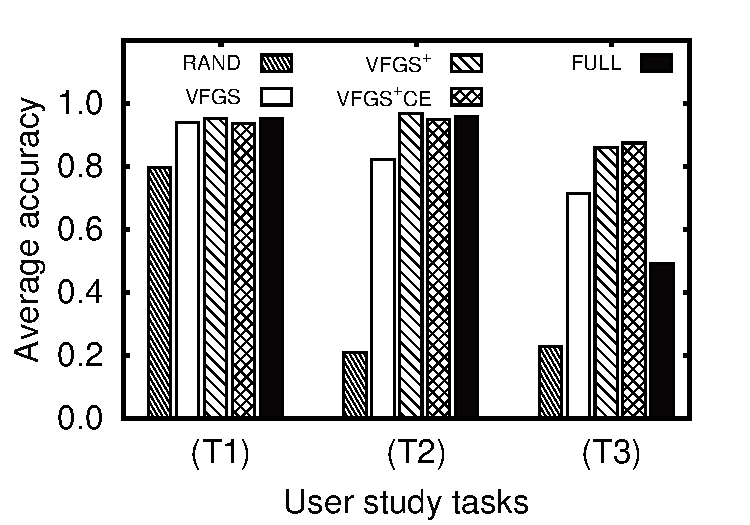
\includegraphics[width=0.3\textwidth]{pictures/userstudy}
	\vspace{-3mm}
	\caption{Average accuracy of the three tasks. X-axis shows different tasks while Y-axis indicates the accuracy.}
	\label{fig:accuracy}
	\vspace{-6mm}
\end{figure}

For (T1) region center identification, the accuracies of our proposals are very similar to that of visualizing the full dataset (i.e., $\full$). In contrast, the accuracy of $\rand{}$ is significantly lower than $\full$. These results suggest that our proposals successfully preserve the centers of human activities even with a low sampling rate of $0.5\%$. $\cavats$ performs slightly worse than $\avats$ and $\full$, and some participants reported that the colors of the trajectories distract them in the post-interview.


%the participants using all the three proposed methods had a very close performance with the participants using whole dataset, indicating the proposed methods can replace the whole dataset with a guaranteed performance in the exploration of human activity center with trajectory visualization.

For (T2) reachable route inspection, $\rand$ has a very low accuracy compared with the other 4 visualization methods. This is because $\rand$ lost many fine-grained details of the trajectories due to uniform sampling, especially in the sparse regions. However, these details can be crucial for determining the existences of a route. Moreover, our advanced methods $\avats$ and $\cavats$ provide noticeably better performance than $\vats$. This is because $\avats$ and $\cavats$ take data distribution and human perception intro consideration, and sample more trajectories in the sparse regions. As a result, more details are preserved.
%It also is worth to point out our $\avats$ (with average accuracy 0.968) outperforms the visualizations of $\full$ (with average accuracy 0.959) slightly.

%Interestingly,
%For the tasks of T2, $\avats$, $\avats$ with color encoding and the whole dataset all have similar accuracy scores which are far higher than random sampling.
%Moreover, $\avats$ and $\avats$ with color encoding also outperforms the $\vats$ clearly by taking the perception parameters into consideration.
% This results demonstrate the advantage of $\avats$ on the urban exploration at a detail level.

(T3) traffic flow comparison is more difficult than T1 and T2, and thus the accuracy drops for all visualization methods. Similar to the case of T1 and T2, $\rand$ has the worst performance among all methods. Remarkably, the accuracies of our proposals (i.e.,  $\vats,\avats$ and $\cavats$) are even higher than $\full$. In the post-interview, the participants reported that $\full$ has severe visual clutter problem, which makes it difficult to compare the traffic flows on two roads. Therefore, the higher accuracies of our proposals indicate that sampling effectively mitigates visual clutter. In addition, the accuracies of $\avats$ and $\cavats$ are higher than that of $\vats$, suggesting that our advanced method and color encoding are effective in alleviating visual clutter.

To sum up, the results in this part shows that our proposals (i.e., ($\vats$, $\avats$, and $\cavats$) are effective in practical spatial tasks. All our methods consistently outperforms $\rand$ by a large margin across different tasks, the advanced methods (i.e., $\avats$, and $\cavats$) often achieve comparable or even better performance than  $\full$.

%\vspace{-2mm}
\subsection{Quantitative Evaluation}\label{sec:quality}
In this part, we quantitatively evaluates our proposals on the \pt{} and \sz{} trajectory datasets from two aspects:
(i) visual fidelity at different zoom levels
and (ii) running time under different sampling rates.

\begin{figure}
 \centering
 \small
 \begin{tabular}{cc}
   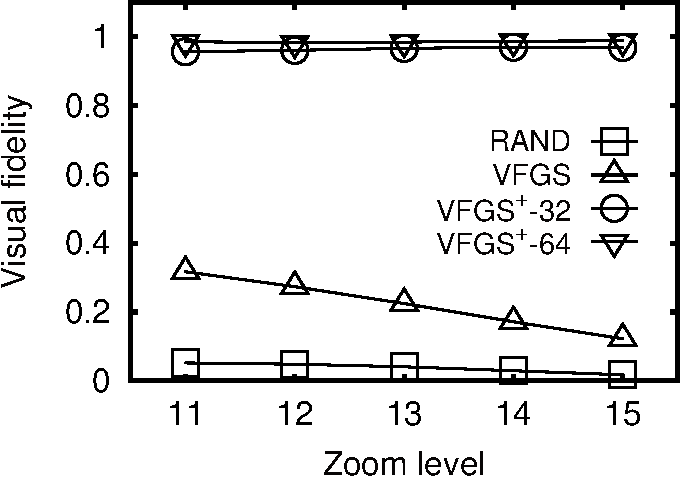
\includegraphics[width=0.44\columnwidth]{pictures/fporto}
   &
   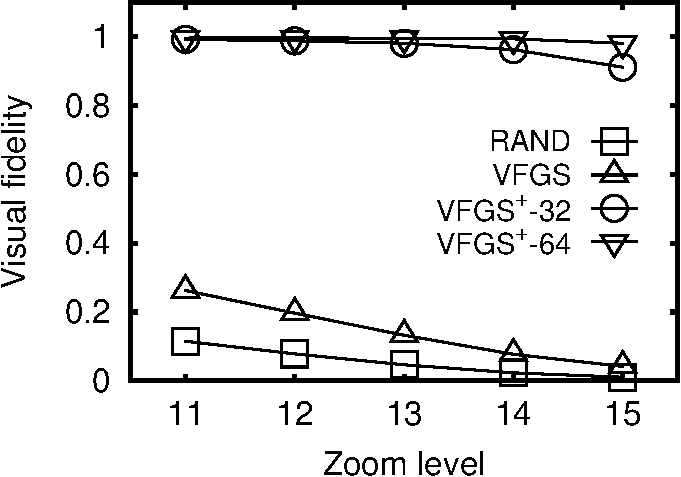
\includegraphics[width=0.44\columnwidth]{pictures/fshenzhen}
   \\
   (A) \pt{}
   &
   (B) \sz{}
 \end{tabular}
 \vspace{-3mm}
 \caption{Visual fidelity vs. zoom levels.}
 \label{fig:fidelity}
 \vspace{-3mm}
\end{figure}

\stitle{Visual fidelity evaluation} We report the \textit{visual fidelity} of different visualization methods in Figure~\ref{fig:fidelity}. Visual fidelity is defined as the $1-loss$, in which $loss$ is the fidelity loss function in Equation~\eqref{eqref:loss}. The sampling rate is $\alpha=0.5\%$ and the visualization using the full dataset is used as the ground-truth. The results show that $\rand$ always has the lowest  visual fidelity. $\vats$ has better visual fidelity than $\rand$ but is significantly outperformed by $\avats$. With $\delta=32$ and $\delta=64$, the minimum visual fidelity values of $\avats$ are 0.95 and 0.91 for \pt{} and \sz{}, respectively. Moreover, the fidelity of all methods increases when the zoom level drops, which in line with Theorem~\ref{the:level}.


%We first evaluate the visual fidelity of our proposed methods.
%We measure the visual fidelity of different approaches over the $\full$ by using the $loss()$ function defined in Section~\ref{sec:def}.
%Figure~\ref{fig:fidelity}(A) and (B) show the visual fidelity of $\rand$, $\vats$, $\avats$ with $\delta=32$ and $\avats$ with $\delta=64$ from zoom level 11 to 15 (i.e., overview to detail view) in
%\pt{} and \sz{}, respectively.
%Results show that $\rand$ does not guarantee the visual fidelity of the result.
%Although $\vats$ offers theoretical visual fidelity guarantee w.r.t. the optimal sampled result set with a given sampling rate, it still has room for improvement over the $\full$;
%Moreover, $\avats$ with $\delta=32$ and $\delta=64$ has excellent visual fidelity w.r.t. the $\full$ dataset. The minimum visual fidelity value is 0.95 and 0.91 in \pt{} and \sz{}, respectively.
%It also confirms the superiority of our proposal.
%The visual fidelity of $\avats$ falls with the rising of zoom levels, e.g., from zoom level 11 to 15.
%The reason is the higher zoom level, the more details are expected.


\begin{figure}
 \centering
 \small
 \begin{tabular}{cc}
   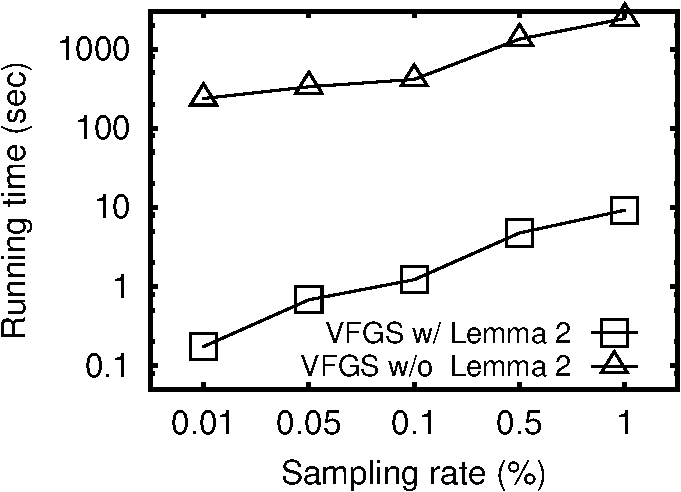
\includegraphics[width=0.44\columnwidth]{pictures/tporto}
   &
   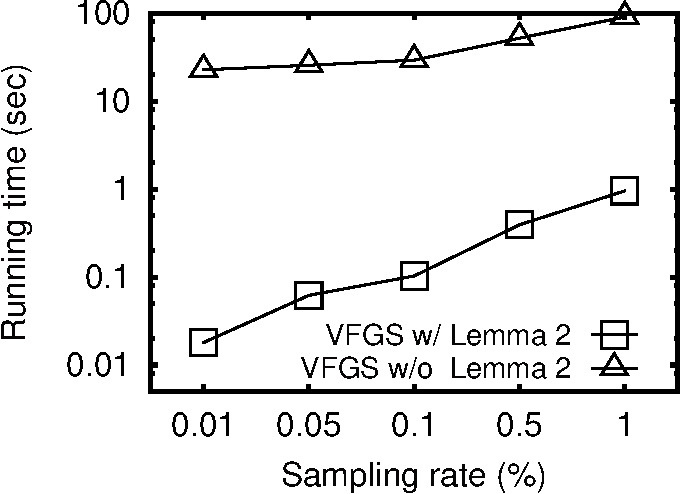
\includegraphics[width=0.44\columnwidth]{pictures/tshenzhen}
   \\
   (A) \pt{}
   &
   (B) \sz{}	
 \end{tabular}
 \vspace{-3mm}
 \caption{Running time of $\vats$ w/ and w/o Lemma~\ref{lem:submodular}.}
 \label{fig:cost}
 \vspace{-3mm}
\end{figure}


\stitle{Running time evaluation} We report the running time of our $\vats$ algorithm in Figure~\ref{fig:cost} by varying the sampling rate from $0.01\%$ to $1\%$. The results show that $\vats$ is quite slow without the submodularity of contribution value, which agrees with Lemma~\ref{lem:submodular} in Section~\ref{sec:opt}.
The optimized $\vats$ (e.g., $\vats$ with Lemma~\ref{lem:submodular}) outperforms $\vats$ by one to three orders of magnitudes on both datasets. The result show that running time of our $\vats$ algorithm is below 1 second in most cases. We have shown that $\vats$ provides good visualization performance with a low sampling rate (e.g., $0.1\%$ or $1\%$) in Section 6.1 and 6.2, and our technical report suggests that the rendering latency scales almost linearly with dataset cardinality. By significantly reducing the dataset cardinality with sampling, $\vats$ can effectively reduces the rendering latency to make interactive visualization possible without sacrificing visual fidelity. For example, rendering the full $\pt{}$ dataset takes about 34 seconds, with a sampling rate of $1\%$, $\vats$ can bring down the rendering latency to less than 1 second.





